This section describes and justifies the design of the ASIC accelerator that will run the vision transformer model. It is split into several sections to describe the
various aspects of the accelerator. A high-level overview of the accelerator is shown in Figure \ref{fig:high_level_arch}. As can be seen, it comprises a single Master
module responsible for interfacing with the host system and number of so-called \ac{cim} modules that perform the actual computation and a shared bus for data and control
signals. For reference, the memory for shared parameters and intermediate results occupies \percentmem{}\% of the area, the compute units occupy \percentcompute{}\% of
the area and the control logic occupies \percentlogic{}\% of the area.

\begin{figure}
    \centering
    \includegraphics[width=0.7\textwidth]{assets/high_level_arch.png}
    \caption{High-level architecture of the ASIC accelerator}
    \label{fig:high_level_arch}
\end{figure}

\subsection{Centralized vs. Distributed Architecture}
The first major design aspect of the accelerator is whether to use a centralized or distributed architecture. A centralized architecture has a single compute unit that
performs all operations and a single memory bank, while a distributed architecture has multiple compute units, each with their own memory. Of course, linear algebra lends
itself very well to parallelization as each \ac{mac} operation is independent of the others. The centralized architecture is simpler to design, has less overhead and lower
area, but is much slower. It is relatively hard to accurately predict the \ac{ppa} of different architectures before implementation. However, designing a distributed
architecture first can be a good starting point as it can easy be scaled up and down to optimize the design. This is the reason this design uses a distributed architecture.

The design uses 64 \ac{cim} to maximize \ac{pe} utilization of the ASIC as mentioned in Section \ref{sec:sw_hw_co-design}

\subsection{Data and Control Bus}
The data and control bus is a bidirectional bus that connects the Master module and all the \ac{cim} modules. Once device may communicate at a each and each is connected to the bus
through tri-state buffers. The bus is 58 bits wide and contains different fields, as summarized in Table \ref{tab:bus_fields}. There are 10 different operations \texttt{Op}, as
described in Appendix \ref{app:bus_ops}. The bus being directly connected to all modules allows for two important features: broadcast and synchronization. There are two types of
broadcast: dense and transpose. Dense broadcast is used to send the same data to all \ac{cim} modules and is used during matrix-matrix multiplications, while transpose broadcast is
used to transpose the matrix (a \ac{cim} holds a row instead of a column). The \ac{cim}s are autonomous with these operations. They do not need do not need involvement from the Master
other than to start the operation. Synchronization is maintained with the \texttt{START\_PISTOL} broadcast, which instructs the \ac{cim}s to go to the next step in their \ac{fsm}.

\begin{table}[ht]
    \centering
    \renewcommand{\arraystretch}{1.2} % Vertical spacing
    \setlength{\arrayrulewidth}{1.5pt} % Thickness of vertical lines
    \caption{Fields of the data and control bus}
    \begin{tabular}{@{} p{1cm}ccc @{}}
        \toprule
        Field           & Width (bits)  & Description \\\midrule
        \texttt{Op}     & 4             & Opcode of the instruction/data \\
        \texttt{ID}     & 6             & ID of the sender or target \ac{cim} \\
        \texttt{Data}   & $3\times16$   & Data (up to 3 $\times$ Q6.10) \\
        \bottomrule
    \end{tabular}
    \label{tab:bus_fields}
\end{table}

\subsection{Master Architecture}
The Master module is responsible for interfacing with the host system. It is a simple module that receives signals from the host microprocessor to start parameter load and
start a new inference. It also interfaces with the external memory holding the parameters and the \ac{adc} in the \ac{eeg} \ac{afe}. It is responsible for directing the \ac{cim}
to perform dense or transpose data broadcasts and for synchronizing their high-level (step-by-step or multi-step) operations.

\subsection{Compute-in-Memory: Architecture}
The \ac{cim} module is the heart of the accelerator. Its architecture is presented in Figure \ref{fig:cim_arch}. It is responsible for performing the actual computation. Each \ac{cim}
module has its own memory for intermediate results and parameters along with control logic and several compute units needed to perform all computation in the model. The \ac{cim} module
is designed to be as autonomous as possible to limit control overhead. It follows the dataflow model of computation, where data is passed from one step of the inference to the next without
Master involvement, unless data needs to be broadcast or transposed across \ac{cim}. The following sections describe different aspects of the \ac{cim} module.
\begin{figure}
    \centering
    \includegraphics[width=0.7\textwidth]{assets/cim_arch.png}
    \caption{Architecture of the Compute-in-Memory module}
    \label{fig:cim_arch}
\end{figure}

\subsection{Compute-in-Memory: Memory}
The \ac{cim} module contains two single-port memory banks: one for intermediate results and one for parameters containing 848 and 528 words, respectively. Having two separate banks
allows for simultaneous read/write to both banks. The memory is generated by ARM's Artisan IP memory compiler and is 65nm 6T SRAM 0.525\si{\square\micro\meter}. It has an aspect ratio of
4, which, as seen in Figures \ref{fig:mem_area} and \ref{fig:mem_overhead}, provides the lowest overhead for the given capacity. The memories are single-cycle. They can also be switched
into a low-power mode when not in use. Table \ref{tab:mem_metrics} shows various metrics of the memory banks for operation at 1.0V and 25\si{\degreeCelsius}.  The \ac{cim} stores lookup
tables for the addresses of the weights and intermediate results in distributed registers. These consume 

\begin{figure}
    \centering
    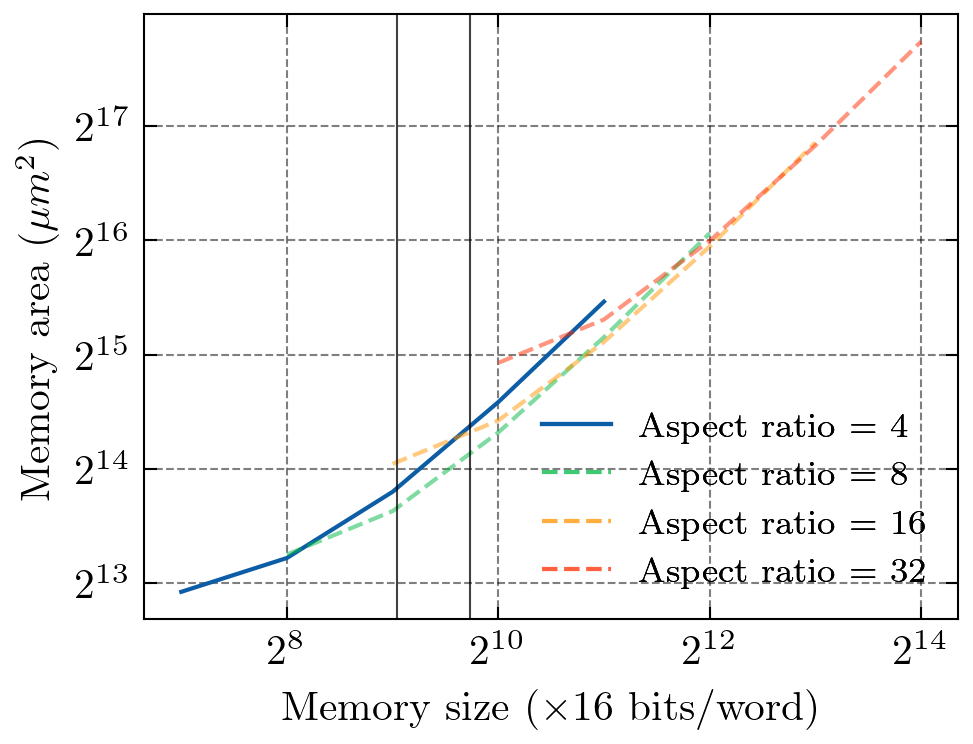
\includegraphics[width=0.7\textwidth]{assets/mem_overhead/mem_area.png}
    \caption{Area of memory banks vs capacity for different aspect ratios}
    \label{fig:mem_area}
\end{figure}
\begin{figure}
    \centering
    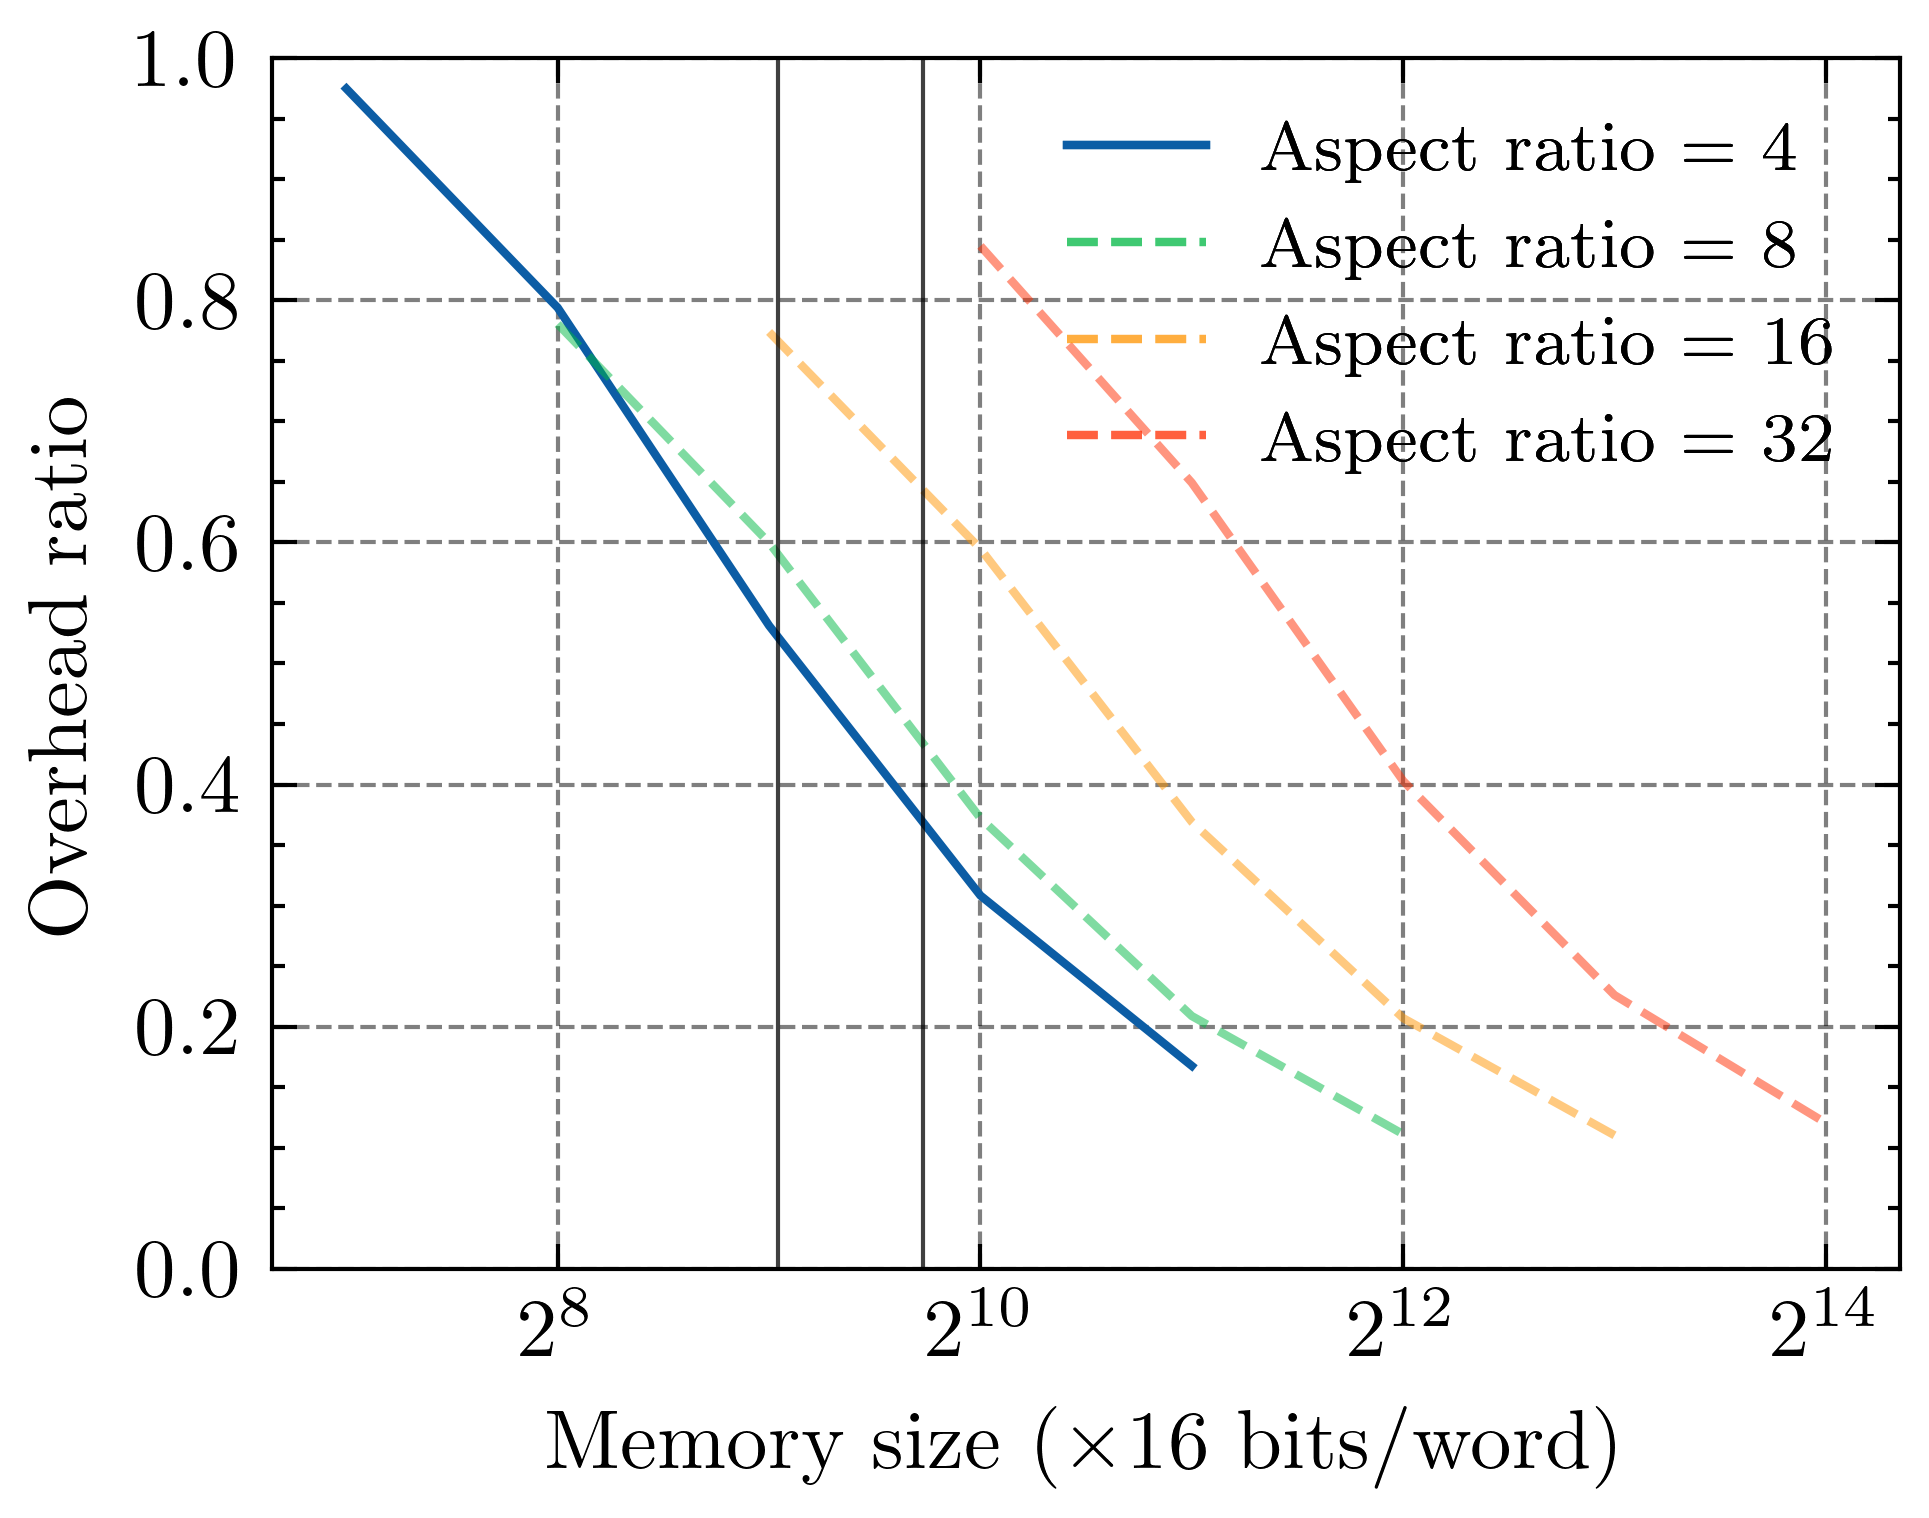
\includegraphics[width=0.7\textwidth]{assets/mem_overhead/mem_overhead.png}
    \caption{Overhead of memory as a fraction of total area for different aspect ratios}
    \label{fig:mem_overhead}
\end{figure}

\begin{table}[ht]
    \centering
    \renewcommand{\arraystretch}{1.2} % Vertical spacing
    \setlength{\arrayrulewidth}{1.5pt} % Thickness of vertical lines
    \caption{Area, leakage power and cycle of the SRAM memory banks}
    \begin{tabular}{@{} p{6cm}ccr @{}}
        \toprule
        Metric                      & 528 words                         & 848 words                         \\\midrule
        Area                        & 16682.54\si{\square\micro\meter}  & 22124.25\si{\square\micro\meter}  \\
        Leakage (nominal)           & 0.122\si{\milli\watt}             & 0.173\si{\milli\watt}             \\
        Leakage (data retention)    & 0.0754\si{\milli\watt}            & 0.055\si{\milli\watt}             \\
        Cycle time                  & 0.852\si{\nano\second}            & 0.865\si{\nano\second}            \\
        \hline
    \end{tabular}
    \label{tab:mem_metrics}
\end{table}

\subsection{Compute-in-Memory: Fixed-Point Accuracy}
All computation in the \ac{cim} module is done in fixed-point format. The model uses Q22.10 format, which has 22 integer bits (including one sign bit) and 10 fractional bits for 
temporary results internal to the compute modules and Q6.10 for storage. This format was chosen because it significantly reduces the area and power consumption of the accelerator compared
to floating-point format. The fixed-point format is also sufficiently accurate for the model. To determine the accuracy of the fixed-point format, an error study was conducted on the
functional simulation. Using the \texttt{fpm} library, all data operations were performed in fixed-point format. The model was ran on a randomly-selected night of sleep data and the output
was compared to the output of the TensorFlow model and the ground truth. Figure \ref{fig:fixed_point_error} shows the error of the fixed-point format compared to the ground truth as a
function of the number of fractional bits (on a 32-bit fixed-point number). As can be seen, the accuracy peaks at 8 bits of fractional precision, only 1.0\% below the accuracy of the
TensorFlow model (which uses 32-bit floating-point format). We can also notice that accuracy drops significantly starting at 19 fractional bits. This is because some intermediate results
overflow when the numbers have less than 12 integer bits, especially because of operations such as \ac{mac}, softmax and LayerNorm, which accumulate numbers over a length of 64. One
limitation of the \texttt{fpm} library is that it can only represent numbers with a total bit count of 4, 8, 16, 32 or 64 bits, so the ideal number of integer bits cannot precisely be
determined. The hardware uses Q8.8 (16-bit) for storage and Q22.10 (32-bit) for computation. The computation format uses more integer bits to avoid overflow errors discussed above and
two additional fractional bits to avoid inaccuracies caused by divide by zeroes.

\begin{figure}
    \centering
    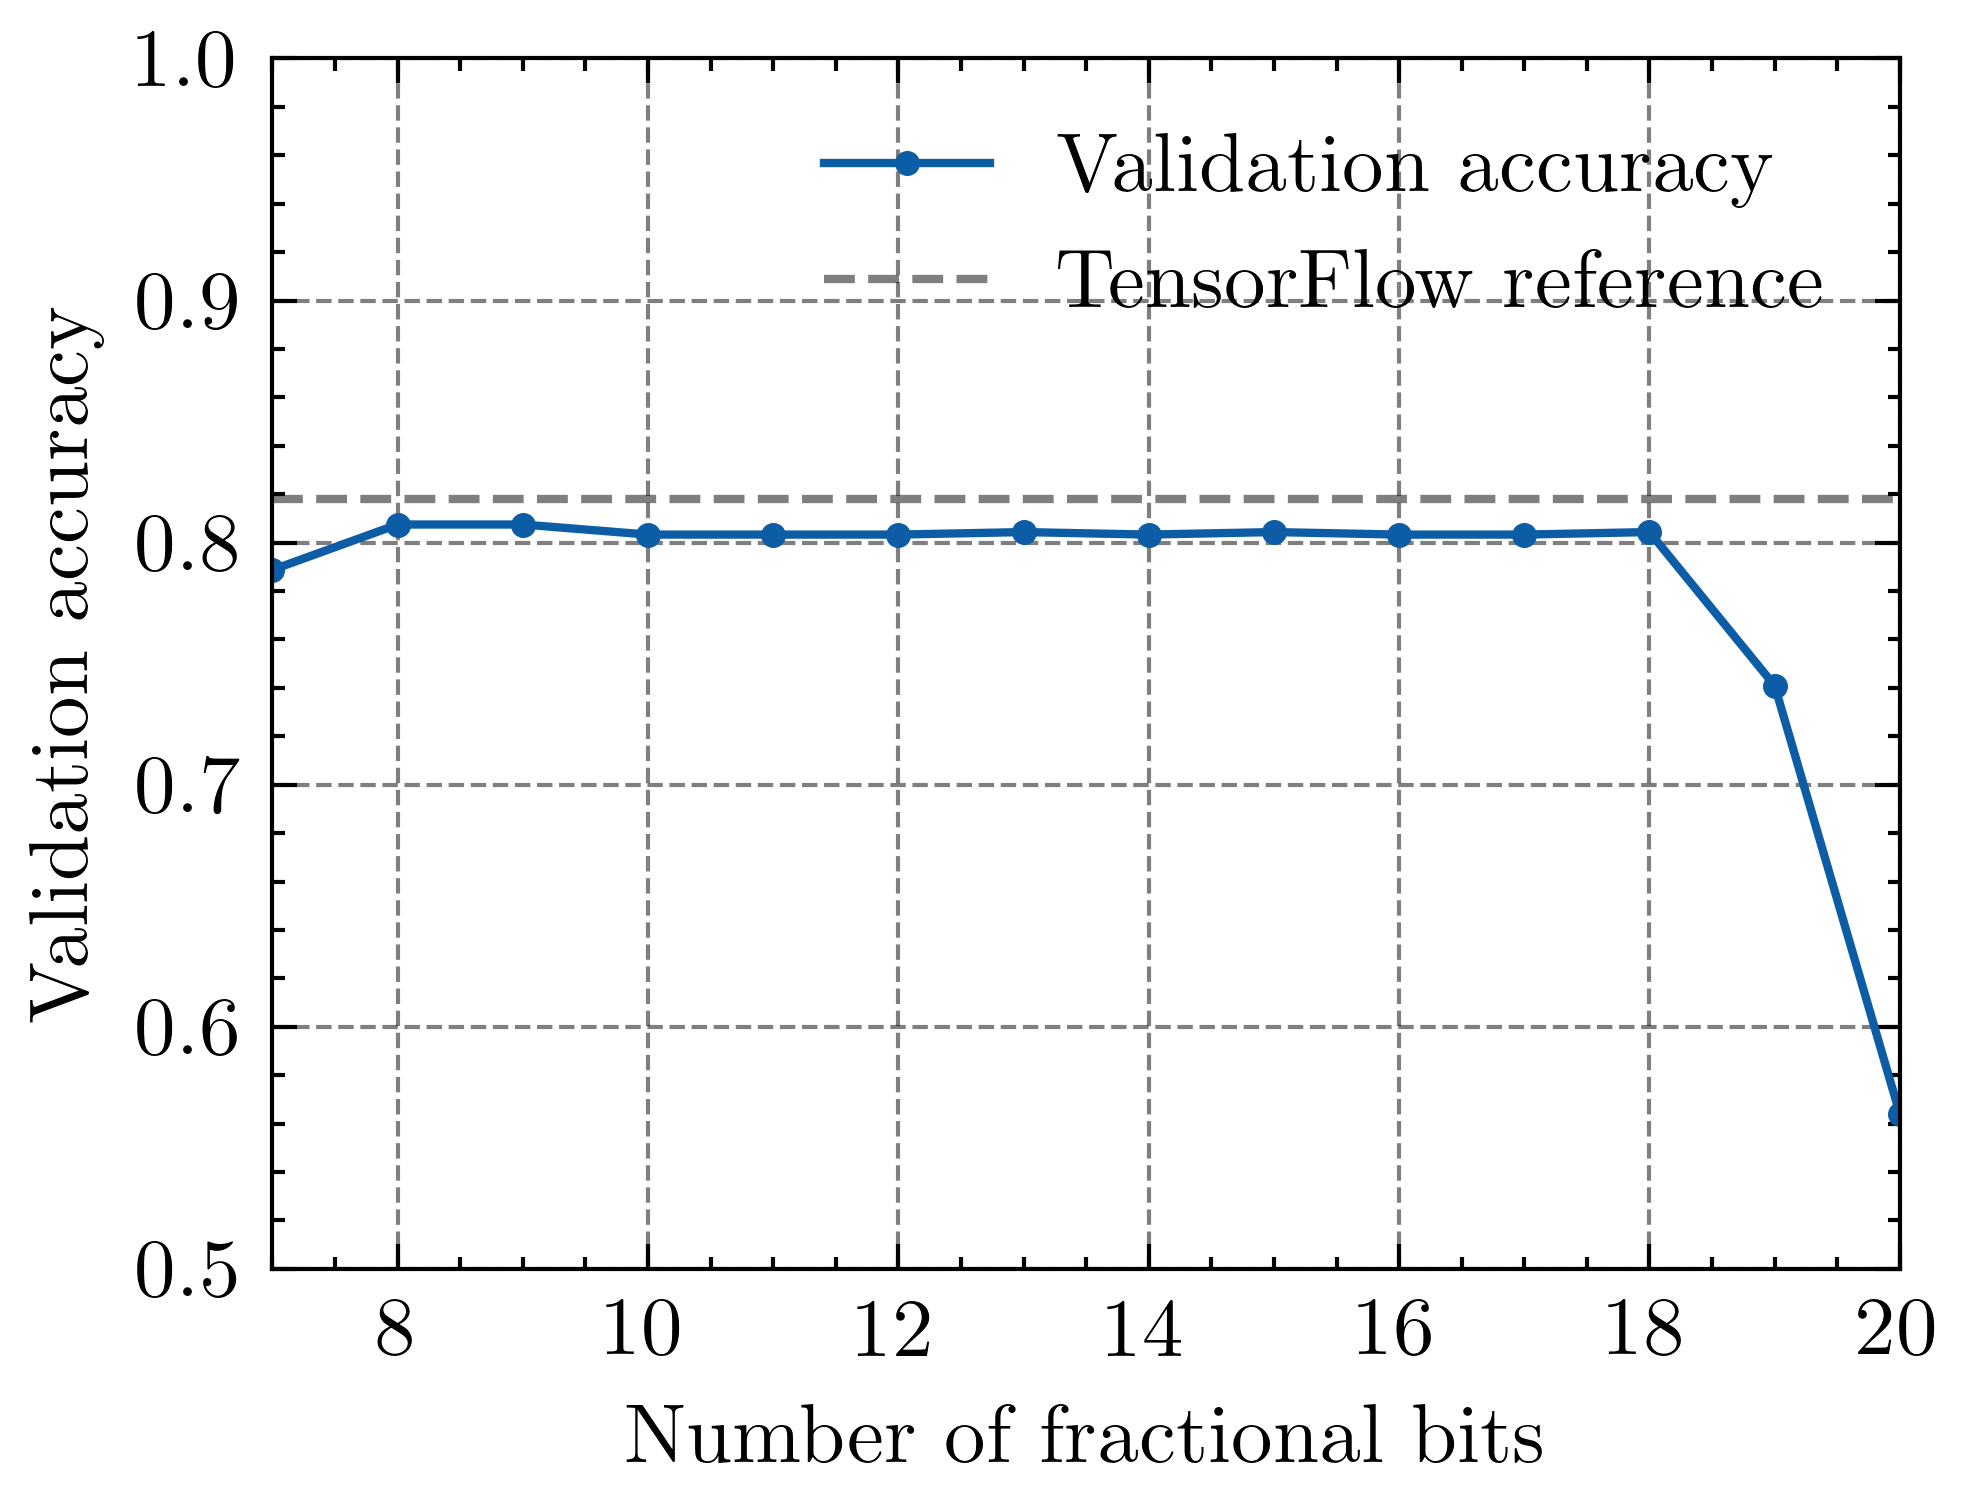
\includegraphics[width=0.7\textwidth]{assets/fixed_point_acc/fixed_point_acc.png}
    \caption{Model accuracy vs number of fractional bits in fixed-point format}
    \label{fig:fixed_point_error}
\end{figure}

\subsection{Compute-in-Memory: Compute Modules}
\label{sec:arch_compute}
This section describes the design and performance metrics of the various compute \ac{ip} modules used in the design. Each is custom-designed for this project.
Each module works with signed (2's complement) fixed-point representation. To avoid overflow, the modules use internal temporary variables of fixed-point format Q22.10.
Table \ref{tab:compute_modules} shows the performance metrics of the compute modules. The working principles of each modules is described briefly in subsequent sections.

\begin{table}[ht]
    \centering
    \renewcommand{\arraystretch}{1.2} % Vertical spacing
    \setlength{\arrayrulewidth}{1.5pt} % Thickness of vertical lines
    \caption{Performance metrics of the compute modules}
    \begin{tabular}{@{} p{2.5cm}ccccc @{}}
        \toprule
        Module                  & Area                              & Cycle/op  & Energy/op                 & Leakage power         & $F_{max}$ \\\midrule
        Adder                   & 450.4\si{\square\micro\meter}     & 1         & 0.99\si{\pico\joule}      & 11.87\si{\micro\watt} & 6.67\si{\giga\hertz} \\
        Multiplier              & 3535.2\si{\square\micro\meter}    & 1         & 7.05\si{\pico\joule}      & 90.50\si{\micro\watt} & 1.59\si{\giga\hertz} \\
        Divider                 & 1719.9\si{\square\micro\meter}    & 35        & 23.44\si{\pico\joule}     & 34.56\si{\micro\watt} & 1.11\si{\giga\hertz} \\
        Exponential             & 2442.2\si{\square\micro\meter}    & 24        & 62.73\si{\pico\joule}     & 47.10\si{\micro\watt} & 7.14\si{\giga\hertz} \\
        Square Root             & 1325.2\si{\square\micro\meter}    & 17        & 18.32\si{\pico\joule}     & 26.30\si{\micro\watt} & 0.758\si{\giga\hertz} \\
        \ac{mac}\footnote[1]    & |                                 & 386       & 820.20\si{\pico\joule}    & |                     & | \\
        \ac{mac}\footnote[2]    & 3129.8\si{\square\micro\meter}    & 391       & 839.32\si{\pico\joule}    & 69.40\si{\pico\joule} & 2.17\si{\giga\hertz} \\
        \ac{mac}\footnote[3]    & |                                 & 456       & 941.68\si{\pico\joule}    & |                     & | \\
        Softmax                 & 2341.1\si{\square\micro\meter}    & 2024      & 1972.5\si{\pico\joule}    & 51.47\si{\micro\watt} & 1.20\si{\giga\hertz} \\
        LayerNorm               & 3836.89\si{\square\micro\meter}   & 1469+494  & 1705.7\si{\pico\joule}    & 78.39\si{\micro\watt} & 0.877\si{\giga\hertz} \\
        \bottomrule
        Total                   & 18780.69\si{\square\micro\meter}  & N/A       & N/A                       & 409.59\si{\micro\watt}& 0.758\si{\giga\hertz} \\
        \hline
    \end{tabular}
    \begin{minipage}{\textwidth}
        \footnotesize
        \noindent\hspace*{1cm}\textsuperscript{1} No activation function applied\\
        \noindent\hspace*{1cm}\textsuperscript{2} Linear activation function applied\\
        \noindent\hspace*{1cm}\textsuperscript{3} Swish activation function applied
    \end{minipage}
    \label{tab:compute_modules}
\end{table}

Note that all measurement in Table \ref{tab:compute_modules} are given for standard 65nm \ac{tsmc} process with a 100MHz clock.
To determine these metrics, the following methodology was used with Synopsys Design Compiler 2017.09 running on UofT's EECG cluster:
\begin{itemize}
    \item Area: Synthesis with the area optimization effort set to \texttt{high}, and the area was extracted from the \texttt{report\_area} command report.
    \item Cycle/op: The latency was observed when running a single operation on a pre-synthesis simulation.
    \item Energy/op: A single-instance testbench running 10000 operations was designed, and a \texttt{.saif} file was generated from the \ac{vcd} dump file of the testbench
    using Synopsys' \texttt{vcd2saif} utility. This provides an average activity factor for each node, yielding an accuracy that is adequate for this discussion. The energy
    per operation was calculated by multiplying the total dynamic power by the time to complete the 10000 operations, divided by 10000.
    \item Leakage power: Synthesis with the power optimization effort set to \texttt{high}, and the leakage power was extracted from the \texttt{report\_area} command report.
    \item $F_{max}$: The \texttt{report\_timing} command was used to determine the maximum frequency of the design.
\end{itemize}

It must be noted that the measurements for all composite compute units (i.e. units that make use of shared resources) \textit{exclude} the area/power/etc. of the shared resources.
Including them would result in misleadingly high figures, given that they are explictly designed to share resources. The total area of the \ac{cim} provides figures more representative
of this integration.

\subsubsection{Adder}
The adder is a single-cycle, combinational module that adds two fixed-point numbers. It uses a ripple-carry adder architecture. The adder has a latency of 1 cycle, which simplifies the logic that uses it.
It also provides an overflow flag. To reduce dynamic power consumption, the adder only updates its output when the \texttt{refresh} signal is high.

\subsubsection{Multiplier}
The multiplier is very similar to the adder. One difference is that it uses Gaussian rounding (also known as banker's rounding). This rounding method rounds 0.5 to the nearest even number. This reduces
the bias in the output that is commonly observed with standard rounding methods, which is particularly important in \ac{mac} operations where the error can accumulate. The multiplier also has a latency of 1
cycle and provides an overflow flag. Like the adder, the multiplier only updates its output when the \texttt{refresh} signal is high.

\subsubsection{Divider}
The divider is more complicated than the adder and multiplier. It performs bit-wise long-division and has a latency of $N+Q+3$ cycles, where $N$ is the number of integer bits and $Q$ is the number of fractional
bits. The divider also provides flags for overflow and divide-by-zero and done/busy status signals. The module start division on an active-high pulse of the \texttt{start} signal and provides the result when the
\texttt{done} signal is high. The divider module is mostly used in the \ac{mac} module during computation of the Swish activation function.

\subsubsection{Exponential}
The exponential module computes the exponential $e^{x}$ of a fixed-point number $x$. It uses a combination of the identities of exponential and a Taylor series approximation around zero to
compute the exponential. Specifically, the module transforms the exponential as such:
\begin{equation}
    e^{x} = 2^{\frac{x}{\ln(e)}} = 2^{z} = 2^{\lfloor{z}\rfloor}2^{z-\lfloor{z}\rfloor}
    \label{eq:exp_transform}
\end{equation}
The compute can then easily compute $2^{\lfloor{z}\rfloor}$ as an inexpensive bit-shift operation and $2^{z-\lfloor{z}\rfloor}$ as a Taylor series approximation. To determine a reasonable
number of terms to use for the Taylor series expansion, an accuracy study was ran. Figure \ref{fig:exp_error} shows the relative error of the exponential module as a function of the order
of the Taylor series expansion for both fixed-point (Q22.10) approximation and float (64b) approximation. As can be seen, the error decreases with an increase in the order of the expansion.
However, for the fixed-point approximation, it converges to a minimum error of \~0.992\%. This is because the quantization of fixed-point dominates the Taylor series error. Therefore,
using a 3rd order Tarlor series expansion to appriximate the exponential function is a good balance between accuracy and latency/energy. Note that these error was measured over the input
range of [-4, 4]. According to the functional simulation, this corresponds to roughly $\pm3$ standard deviations from the mean of inputs to the exponential function. To further speed up the
computation, the exponential module uses a lookup table to store the Taylor series coefficients as well as $1/ln(e)$. To reduce area, the exponential module does not instantiate its own adder and
multiplier modules. Rather, it accesses the adder and multiplier modules in the \ac{cim} module shared with other compute units. The latency is 24 cycles.

\begin{figure}
    \centering
    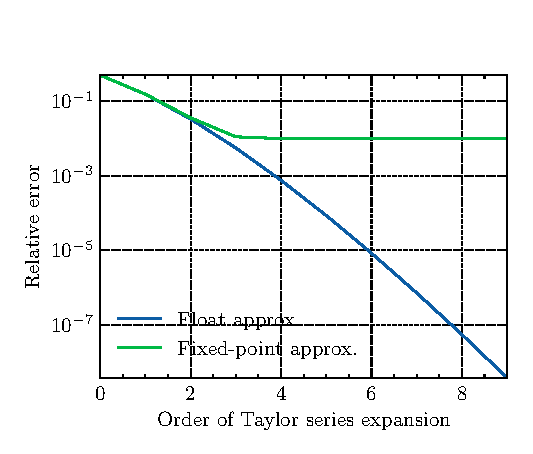
\includegraphics[width=0.7\textwidth]{assets/exp_approx_error/exp_approx_error.eps}
    \caption{Approximation error of the exponential vs Taylor series expansion order}
    \label{fig:exp_error}
\end{figure}

\subsubsection{Square Root}
The square root module computes the square root of a fixed-point number using an iterative algortihm. It has a latency of $(N+Q)//2+1$ cycles, where $//$ denotes integer division. The module provides flags for overflow and
negative radicand and start/busy/done signals. The module starts computation on an active-high pulse of the \texttt{start} signal and provides the result when the \texttt{done} signal is high.

\subsubsection{Multiply-Accumulate}
The \ac{mac} module performs a vector dot-product for a given pair of base addresses for the data and length of the vector and applies a selectable activation function to the result. Similar to the exponential module, it
uses shared adder, multiplier, divider and exponential modules in the \ac{cim} module. It can implement three activation functions: none, linear and Swish. For a nominal length of 64 (which corresponds to the embedding
depth of the model, a very common value for matrix dimensions in the model) and Q22.10 formate, the latencies are 386, 391 and 456, respectively. Note that, although the Swish activation function comprises a divider operation,
the \ac{mac} compute latency can still be kept fairly short because the divisor is the same for all elements. The module can thus perform the division once and multiply by the inverse, which is a single-cycle operation.Finally,
the \ac{mac} module can be directed to choose the second vector from weights or intermediate results memory.

\subsubsection{Softmax}
The softmax module computes the softmax function of a vector of fixed-point numbers. Similarly to the \ac{mac} module, it uses shared adder, mulitplier, divider and exponential modules and provides \texttt{busy} and
\texttt{done} signals. For a 64-element Q22.10 vector, the latency is 2024 cycles. This is significantly longer than other vector compute modules such as the \ac{mac} because, in the softmax operation, each element is exponantiated
individually.

\subsubsection{LayerNorm}
The final compute module is the LayerNorm module. It computes the Layer Normalization of a vector of fixed-point numbers. As described in section \ref{sec:vision_transformer}, the LayerNorm operation consists of a normalization of
the vector on the horizontal dimension followed by scaling and shifting using learnable parameters on the vertical dimension. Because each \ac{cim} module stores one vector at a time, the LayerNorm operation must be separated into
two stages with a matrix transpose broadcast between the two. The latency for the first half is 1469 cycles and the latency for the second half is 494 cycles. The module provides \texttt{busy} and \texttt{done} signals and is controlled
with a \texttt{half-select} and \texttt{start} pulse signals. Because the length of the vector is constrained to be a power of two, the module uses bit-shifting instead of division for the normalization operation to decrease latency and energy
per operation.

\subsection{Clock Gating}
This design makes use of clock gating, which is a technique to reduce dynamic power consumption by disabling the clock signal to modules that are not in use. This is handled automatically by the Synopsys Design Compiler tool.
